\chapter{Statistical methods}\label{ch:stat}

In the course of analyzing the data sets provided by the CMS experiment and used in this thesis, several statistical tools have been employed; in this chapter, a description of these tools will be presented, starting with the general statement of the multivariate analysis method, followed by the particularities of the Boosted Decision Trees (BDT) method and its application to the classification problem. Statistical inference methods used will also be presented. This chapter is based mainly on the references \cite{mva, tmva, luca}.      

\section{Multivariate analysis}\label{sec:mva}

Multivariate data analysis (MVA) makes reference to statistical techniques that analyze data containing information of more than one variable, commonly taking into account the effects of all variables on the response of the particular variable under investigation, \ie, considering all the correlations between variables. MVA is employed in a variety of fields like consumer and market research, quality control and process optimization. From a MVA it is possible to identify the dominant patterns in the data, like groups, outliers and trends, and determine to which group a set of values belong; in the particle physics context, MVA methods are used to perform the selection of certain type of events, from a large data set, using a potentially large number of measurable properties for each event.

Processes with small cross section, as the \tHq process, normally are hidden behind more common processes; therefore, the data set results in a subset of events with characteristic features of interest (signal) mixed in randomly with a much larger number of SM events that can mimic these features of interest (background) which implies that it is not possible to say with certainty that a given event is signal or background. In that sense, the problem can be formulated as one where a set of events have to be classified according to some features; these features correspond to the measurements of several parameters like energy or momentum, organized in a set of \textit{input variables}. The measurements for each event can be written in a vector $\textbf{x}=(x_1,.....,x_n)$ for which

\begin{itemize}
\item Signal hypotheses $\to f(\textbf{x}|s)$ is the probability density (\ti{likelihood function}) that $\textbf{x}$ is the set of measured values given that the events is a signal event. 
\item Background hypotheses $ \to f(\textbf{x}|b)$ is the probability density (\ti{likelihood function}) that $\textbf{x}$ is the set of measured values given that the event is a background event.
\end{itemize}

Figure \ref{fig:scatter_plot} shows three ways to perform a classification of events for which measurements of two properties, two input variables, have been performed; blue circles represent signal events while red triangles represent background events. The classification on (a) is \textit{cut-based} requiring $x_1<c_1$ and $x_2<c_2$; usually the cut values are chosen according to some knowledge about the event process. In (b), the classification is performed by stating a cut involving a linear function of the input variables and so the boundary, while in (c) the the relationship between the input variables is not linear thus the boundary is not linear either.          

\begin{figure}[!h]
  \centering
  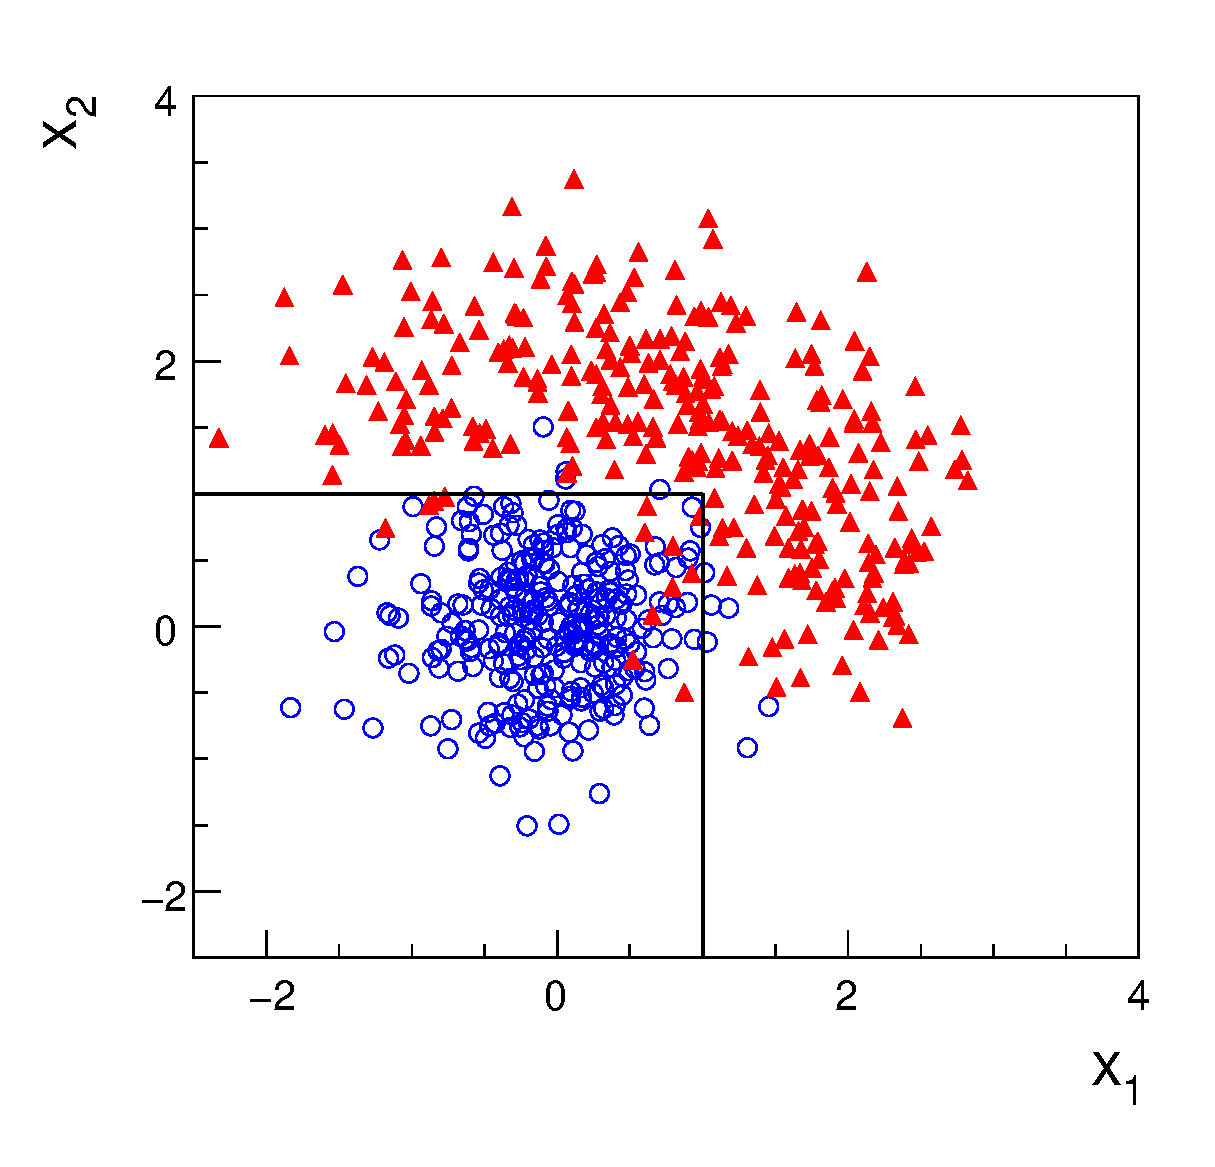
\includegraphics[width=4.5cm,height=4.5cm]{Cuts}
  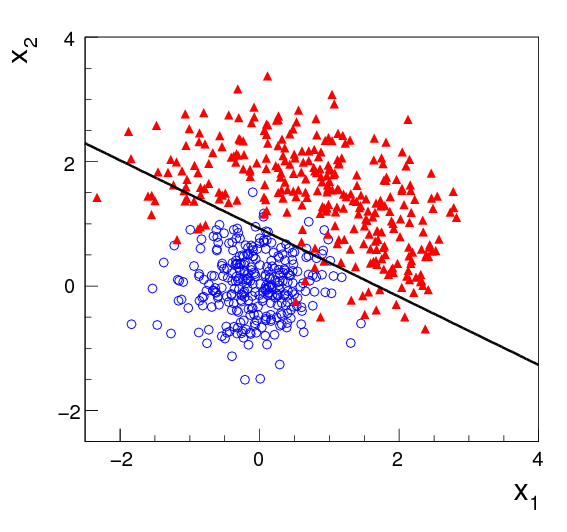
\includegraphics[width=4.5cm,height=4.5cm]{Fisher}
  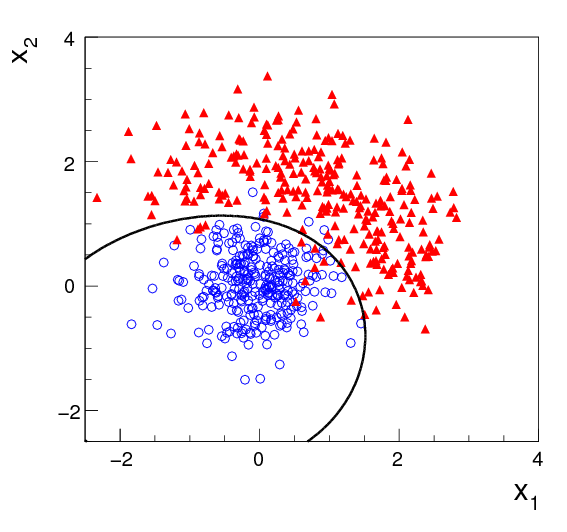
\includegraphics[width=4.5cm,height=4.5cm]{SVM05}
  \caption[Scatter plots-MVA event classification.]{Scatter plots-MVA event classification. Distribution of two input variables $x_1$ and $x_2$ measured for a set of events; blue circles represent signal events and red triangles represent background events. The classification is based on (a) cuts, (b) linear boundary, and (c) nonlinear boundary\cite{mva}}\label{fig:scatter_plot}
\end{figure}

The boundary can be parametrized in terms of the input variables such that the cut is set on the parametrization instead of on the variables, \ie, $y(\textbf{x})=y_{cut}$ with $y_{cut}$ a constant; thus, the acceptance or rejection of an event is based on what side of the boundary is the event located. If $y(\textbf{x})$ has functional form, it can be used to determine the probability distribution functions $p(y|s)$ and $p(y|b)$ and then perform a scalar test statistic with a single cut on the scalar variable $y$. 

\begin{figure}[!h]
  \centering
  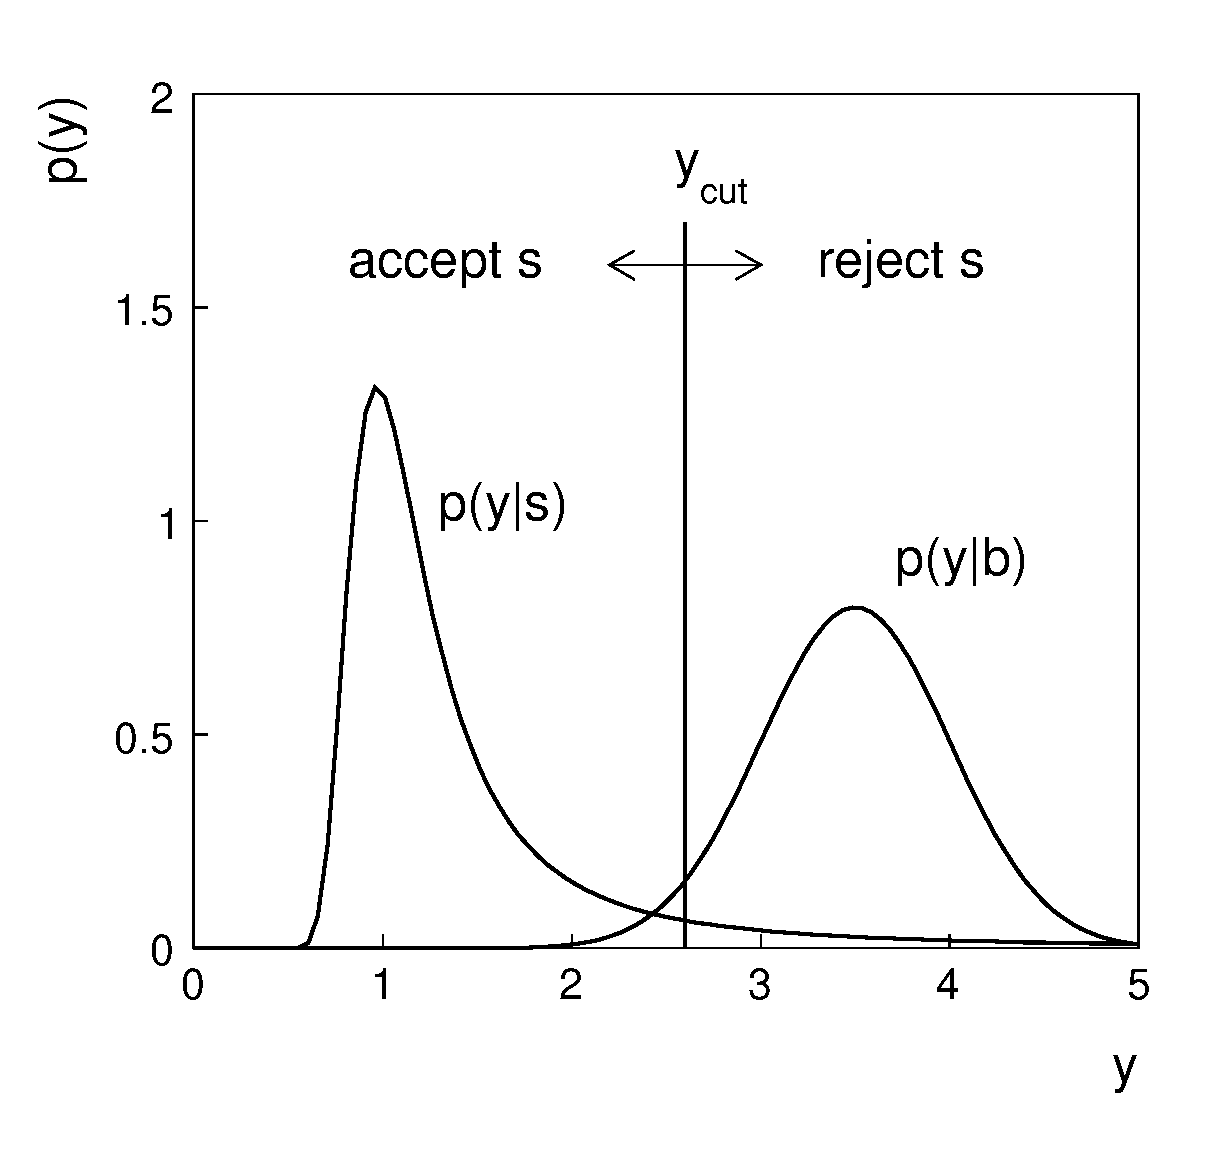
\includegraphics[scale=0.4]{TestStat}
  \caption[Scalar test statistical.]{Distributions of the scalar test statistic $y(\textbf{x})$ under the signal and background hypotheses.\cite{mva}}\label{fig:scalar_test}
\end{figure}

Figure \ref{fig:scalar_test} illustrates what would be the probability distribution functions under the signal and background hypotheses for a scalar test statistic with a cut on the classifier $y$. Notice that the tails of the distributions indicate that some signal events fall on the rejection region and some background events fall on the acceptance region; therefore, it is convenient to define the \textit{efficiency} with which events of a given type are accepted, thus, the signal and background efficiencies are given by 

\begin{eqnarray}
\label{eq:sigeff}
\varepsilon_{\textrm{s}} & = & P( \mbox{accept event} | \mbox{s} ) = \int_{\textrm{A}} f(\textbf{x} | \mbox{s} ) \, d \textbf{x} = \int_{-\infty}^{y_{\textrm{cut}}} p(y | \mbox{s}) \, dy\;, \\*[0.3 cm]
\varepsilon_{\textrm{b}} & = & P( \mbox{accept event} | \mbox{b} ) = \int_{\textrm{A}} f(\textbf{x} | \mbox{b} ) \, d \textbf{x} = \int_{-\infty}^{y_{\textrm{cut}}} p(y | \mbox{b}) \, dy \;,
\end{eqnarray}

\noindent where A is the acceptance region. Under these conditions, the background hypothesis corresponds to the \textit{null hypothesis ($H_0$)}, the signal hypothesis corresponds to the \textit{alternative hypothesis ($H_1$)}, the background efficiency is the significance level of the test, and signal efficiency is the power of the test; what is sought in an analysis is to maximize the power of the test relative to the significance level.

\subsection{Decision trees }

For this thesis, the implementation of the MVA strategy, described above, is performed through decision trees by using the TMVA software package \cite{tmva} included in the the ROOT analysis framework\cite{root}. In a simple picture, a decision tree classifies events according to their input variables values by setting a cut on each input variable and checking which events are on which side of the cut, just as proposed in the MVA strategy, but in addition, as a machine learning algorithm, decision trees offer the possibility to be trained and then perform the classification efficiently.    

\begin{figure}[!h]
  \centering
  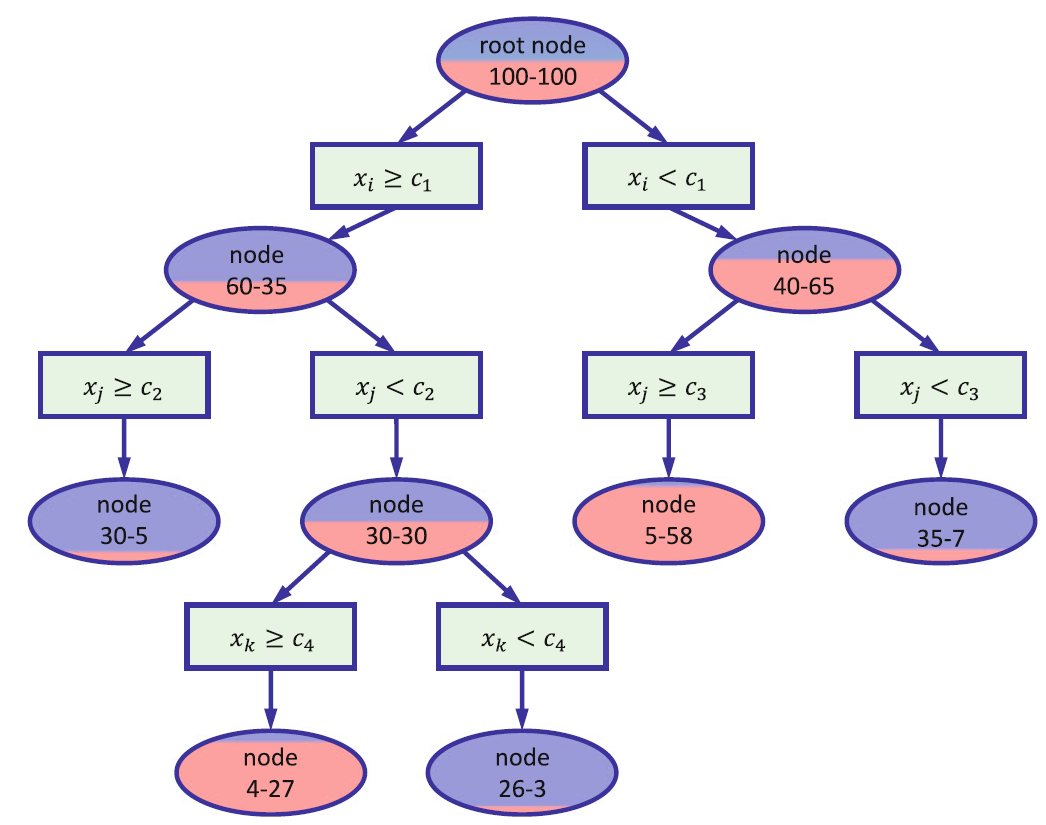
\includegraphics[scale=0.4]{decision_tree}
  \caption[Decision tree.]{Example of a decision tree. Each node is fed with a MC sample mixing signal and background events (left-right numbers); nodes colors represent the relative amount of signal/background events \cite{luca}.}\label{fig:dt}
\end{figure}

The training or growing of a decision tree is the process that defines the rules for classifying events; this process is represented in figure\ref{fig:dt} and consist of several steps

\begin{itemize}
\item take MC samples of signal and background events and split them into two parts each; first parts form the training sample which will be used in the decision tree training, while the second parts form the test sample which will be used for testing the final classifier obtained from the training. Each event has associated a set of input variables $\textbf{x}=(x_1,.....,x_n)$ which serve to distinguish between signal and background events. The training sample is taken in at the root \textit{node}. 
\item pick one variable, say $x_i$
\item pick one value of $x_i$, each event has its own value of $x_i$, and split the training sample into two subsamples $B_1$ and $B_2$; $B_1$ contains events for which $x_i< c_1$ while $B_2$ contains the rest of the training events;
\item scan all possible values of $x_i$ and find the splitting value that provides the \textit{best} classification\footnote{ Quality of the classification will be treated in the next paragraph.}, \ie, $B_1$ is mostly made of signal events while $B_2$ is mostly made of background events.
\item It is possible that variables other than the picked one produce a better classification, hence, all the variables have to be evaluated. Pick the next variable, say $x_j$, and repeat the scan over its possible values.
\item At the end, all the variables and their values will have been scanned, the \textit{best} variable and splitting value will have been identified, say $x_1, c_1$, and there will be two nodes fed with the subsamples $B_1$ and $B_2$. 
\end{itemize}

Nodes are further split by repeating the decision process until: a given number of final nodes is obtained, nodes are largely dominated by either signal or background events, or nodes has too few events to continue. Final nodes are called \textit{leaves} and they are classified as signal or background leaves according to the class of the majority of events in them. Each \textit{branch} in the tree corresponds to a sequence of cuts. 

The quality of the classification at each node is evaluated through a separation criteria; there are several of them but the \textit{Gini Index (G)} is the one used in the decision trees trained for the analysis in this thesis. G is written in terms of the purity (P), \ie the fraction of signal events, of the samples after the separation is made; it is given by
\beqn
G=P(1-P)
\eeqn
\noindent notice that P=0.5 at the root node while G=0 for pure leaves. For a node $A$ split into two nodes $B_1$ and $B_2$ the G gain is
\beqn
\Delta G = G(A)- G(B_1)-G(B_2)
\eeqn

\noindent the \textit{best} classification corresponds to that for which the gain of G is maximized; hence, the scanning over all event's variables and their values is of capital importance.

In order to provide a numerical output for the classification, events in a signal(background) leaf are assigned an score of 1(-1) each, defining in this way the decision tree \textit{classifier or weak learner} as

\[
f(\textbf{x}) = \left\{
\begin{array}{ll}
  1  &  \textbf{x} \quad \textrm{in signal region,}\\
  -1 &  \textbf{x} \quad \textrm{in background region.}
\end{array}
\right.
\]

Figure \ref{fig:dtr}shows an example of the classification of a sample of events, containing two variables, performed by a decision tree.

\begin{figure}[!h]
  \centering
  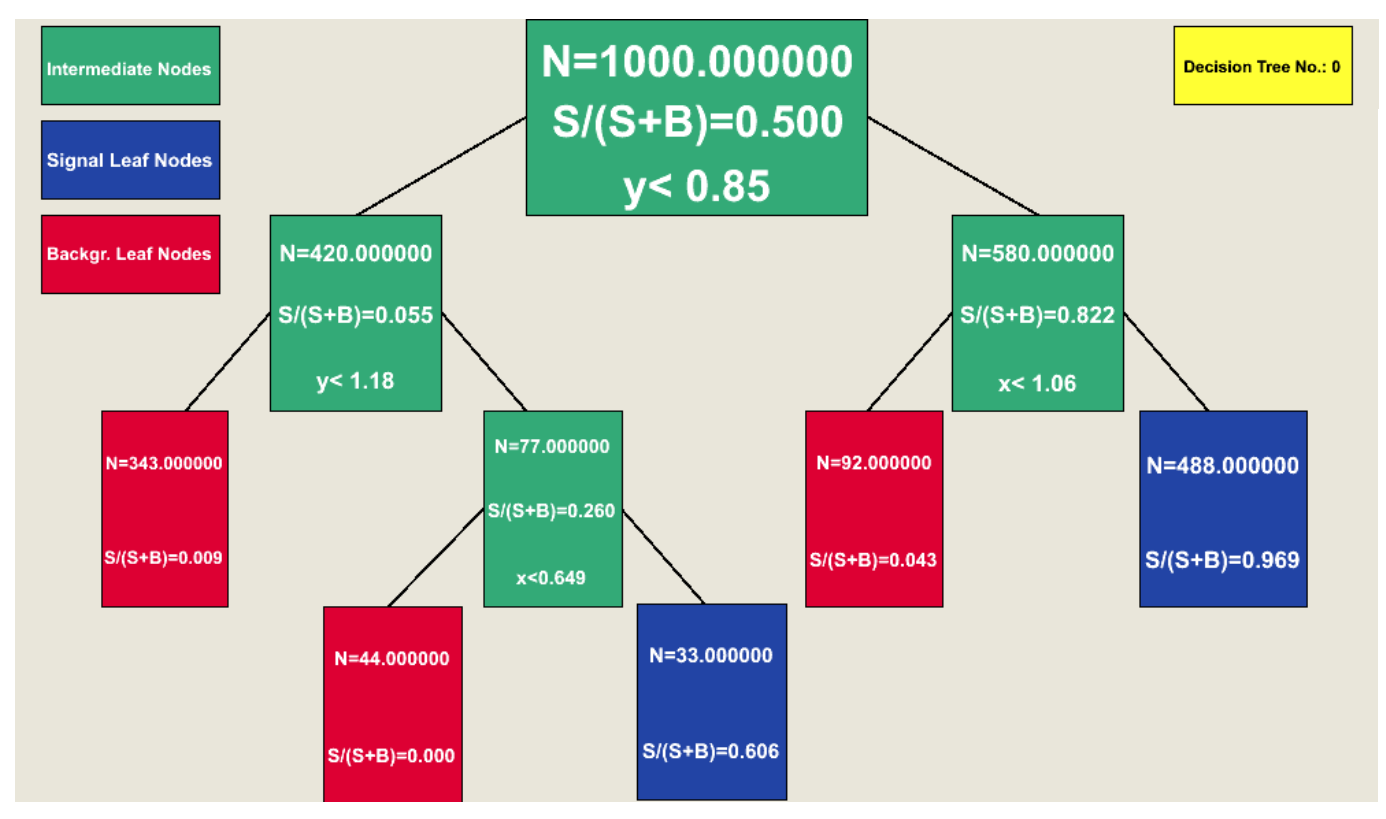
\includegraphics[scale=0.38]{dt1}
  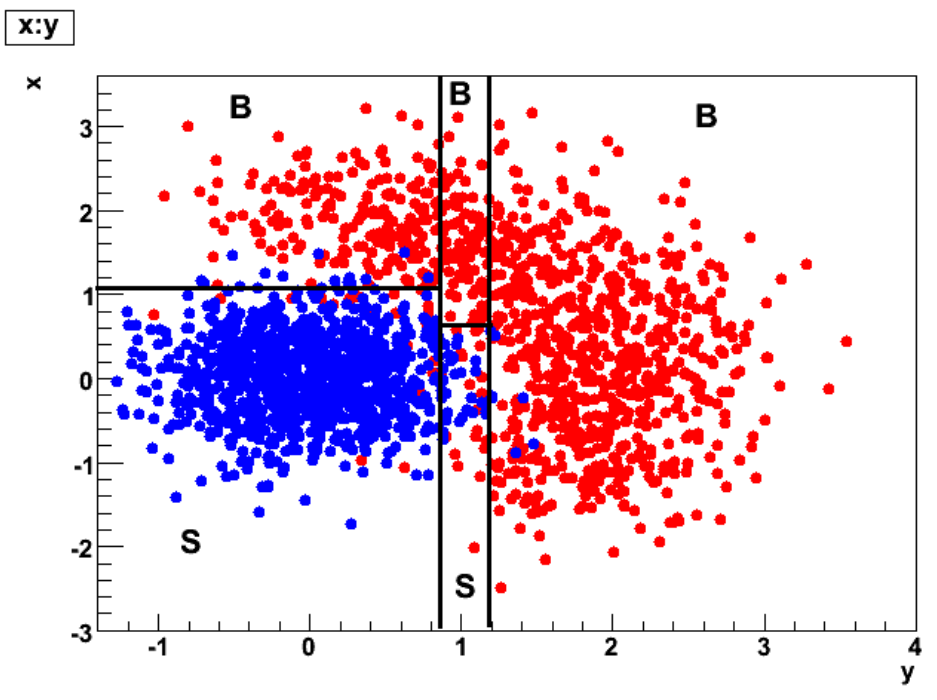
\includegraphics[scale=0.38]{dt2}
  \caption[Decision tree output example.]{Example of a decision tree output. Each leaf, blue for signal events and red for background events, represent a region in the variables phase space \cite{coadou}.}\label{fig:dtr}
\end{figure}

\subsection{Boosted decision trees (BDT).}

Event misclassification occurs when a training event ends up in the wrong leaf, \ie, a signal event ends up in a background leaf or a background event ends up in a signal leaf. A way to correct it is to assign a weight to the misclassified events and train a second tree using the reweighted events; the event reweighting is performed by a boosting algorithm, events with increased weight are known as \textit{boosted} events, in such a way that when used in the training of a new decision tree they get correctly classified. The process is repeated iteratively adding a new tree to a forest and creating a set of classifiers which are combined to create the next classifier; the final classifier offers more stability\footnote{Decision trees suffer from sensitivity to statistical fluctuations in the training sample which may leads to very different results with an small change in the training samples.} and has a smaller misclassification rate than any individual ones. The resulting tree collection is known as a \textit{boosted decision tree (BDT)}.

Thus, purity of the sample is generalized to 

\beqn
P=\frac{\sum_s w_s}{\sum_s w_s + \sum_b w_b}
\eeqn

\noindent where $w_s$ and $w_b$ are the weights of the events; the Gini index is also generalized

\beqn
G=\left(\sum_i^n w_i\right) P(1-P)
\eeqn

\noindent with n the number of events in the node. The final score of an event, after passing through the forest, is calculated as the renormalized sum of all the individual (possibly weighted) scores; thus, high(low) score implies that the event is most likely signal(background).   

The boosting procedure, implemented in the  \textit{Gradient boosting} algorithm used in this thesis, produce a classifier $F(\textbf{x})$ which is the weighted sum of the individual classifiers obtained after each iteration,\ie,   

\beqn
F(\textbf{x})=\sum_{m=1}^M \beta_m f(\textbf{x};a_m)
\eeqn

\noindent where M is the number of trees in the forest. The \textit{loss function $L(F,y)$} represent the deviation between the classifier $F(\textbf{x})$ response and the true value $y$ obtained from the training sample (1 for signal events and -1 for background event), according to 

\beqn
L(F,y)= \textrm{ln}(1+ e^{-2F(\textbf{x})y})
\eeqn

\noindent thus, the reweighting is employed to ensure the minimization of the loss function; a more detailed description of the minimization procedure can be found in reference \cite{friedman}. The final classifier output is later used as a final discrimination variable, labeled as \ti{BDT output/response}.

\subsection{Overtraining.}

Decision trees offer the possibility to have as many nodes as wished in order to reduce the misclassification to zero (in theory); however, when a classifier is too much adjusted to a particular training sample, the classifier response to a slightly different sample may leads to a completely different classification results; this effect is know as \ti{overtraining}.

An alternative to reduce the overtraining in BDTs consist in prunning the tree by removing statistically insignificant nodes after the tree growing is completed but this option is not available for BDTs with gradient boosting in the TMVA-toolkit, therefore, the overtraining has to be reduced by tuning the algorithm, number of nodes, minimum number of events in the leaves, etc. The overtraining can be evaluated by comparing the responses of the classifier when running over the training and test samples.   

\subsection{Variable ranking.}

BDTs have the couple of particular advantages related to the input variables; on one side, they are relatively insensitive to the number of input variables used in the vector \textbf{x}. The ranking of the BDT input variables is determined by counting the number of times a variable is used to split decision tree nodes; in addition, the separation gain-squared achieved in the splitting and the number of events in the node are accounted by applying a weighting to that number. Thus, those variables with small or no power to separate signal and background events are rarely chosen to split the nodes,\ie, are effectively ignored.

On the other side, variables correlations play an important role for some MVA methods like the Fisher discriminant algorithm in which the first step consist of performing a linear transformation to a phase space where the correlations between variables are removed; in case of BDT algorithm, correlations do not affect the performance.

\subsection{BDT output example.}

\begin{figure}[!h]
  \centering
  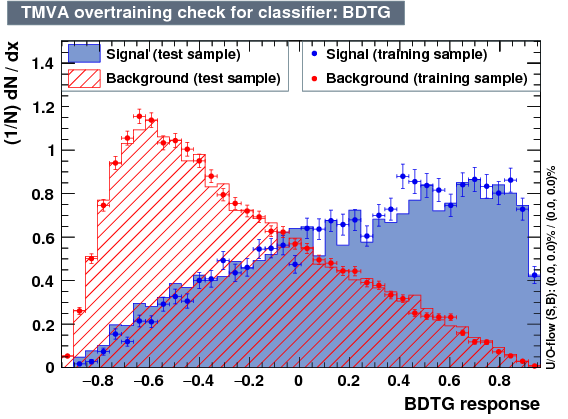
\includegraphics[scale=0.5]{bdt_output}
  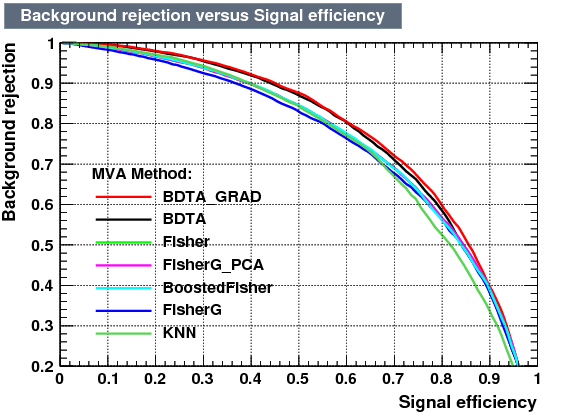
\includegraphics[scale=0.5]{roc_multimva}
  \caption[BDT output example.]{Left: Output distributions for the gradient boosted decision tree (BDTG) classifier using a sample of signal(\pp $to$ \tHq ) and background(\pp $\to$ \ttbar) events. Right: Background rejection vs signal efficiency (ROC curves) for various MVA classifiers running over the same sample used to produce the plot on the left.}\label{fig:bdt_output}
\end{figure}


Left side of figure \ref{fig:bdt_output} shows the BDT output distributions for signal(\pp $\to$ \tHq ) and background(\pp $\to$ \ttbar) events; this plot is the equivalent to the one showed in figure \ref{fig:scalar_test}. A forest with 800 trees, maximum depth per tree = 3, and gradient boosting have been used as training parameters. The BDTG classifier offers a good separation power; while there is a small overtraining in the signal distribution, the background distribution seems to be well predicted which might indicate that the sample is composed of more background than signal events.

Right side of figure \ref{fig:bdt_output} shows the background rejection vs signal efficiency curves for several combinations of MVA classifiers-boosting algorithms; these curves are known as ROC curves and give an indication of the performance of the classifier. The best performance is achieved with the BDTG classifier (BDTA\_GRAD).   


\section{Statistical inference.}

Once events are classified, the next step consists in finding the parameters that define the likelihood functions $f(\textbf{x}|s), f(\textbf{x}|b)$ for signal and background events respectively. In general, likelihood functions depend not only on the measurements but also on parameters ($\theta_m$) that define their shapes; the process of estimating these \ti{unknown parameters} and their uncertainties from the experimental data is called \ti{inference}. The likelihood function for N the events the in a sample is the combination of all the likelihoods functions

\beqn
L(\bm{\theta})=\prod_{i=1}^N f(\textbf{x}^i|\bm{\theta})=\prod_{i=1}^N f(x^i_1,...,x_n^i;\theta_1,...,\theta_m)\label{eqn:ml}
\eeqn

Thus, the estimation of the unknown parameters from experimental data samples is written in terms of a central value using the notation

\beqn
\theta=\hat{\theta}\pm\delta \theta  
\eeqn

where the interval $[\hat{\theta}+\delta \theta, \hat{\theta}-\delta \theta]$ is called \ti{confidence interval}; it is usually interpreted, in the limit of infinite number of experiments, as the interval where the true value of the unknown parameter $\theta$ is contained with a probability of 0.6827 (if no other convention is stated).  

\subsection{Nuisance parameters.}

The unknown parameter vector $\bm{\theta}$ is made of two types of parameters: on one side, those parameters that provide information about the physical observables of interest for the experiment (\ti{parameters of interest}); on the other side, the \ti{nuisance parameters} that are not of direct interest for the experiment but that needs to be included in the analysis in order to achieve a satisfactory description of the data. They represent effects of the detector response like the finite resolutions of the detection systems, miscalibrations, and in general any source of uncertainty introduced in the analysis.

In some cases the nuisance parameters are estimated using dedicated data samples, for instance data from test beams for calibration purposes, when MC samples are not suitable. The nuisance parameter uncertainties produce \ti{systematic uncertainties} while the uncertainties associated to fluctuations in data and related to the estimation of the parameters of interest produce \ti{statistical uncertainties}.

\subsection{Maximum likelihood estimation method}

The function that produce the estimate of a parameter is called \ti{estimator}, therefore, estimators are usually constructed using mathematical procedures encoded in algorithms. The estimation method used in this thesis is the \ti{Maximum Likelihood Estimation} method (MLE); it is based on the combined likelihood function defined by eqn. \ref{eqn:ml} and the procedure seeks for the parameter set that corresponds to the maximum value of the combined likelihood function, \ie, the \ti{maximum likelihood estimator} of the unknown parameter vector $\bm{\theta}$ is the function that produce the vector $\bm{\hat \theta}$ for which the likelihood function $L(\bm{\theta})$ evaluated at the measured sample $\textbf{x}$ is maximum.  

Usually, the logarithm of the likelihood function is used in the numerical algorithms implementations in order to avoid underflow the numerical precision of the computers due to the product of low likelihoods. In addition, it is usual minimize the negative logarithm of the likelihood function instead of maximizing the logarithm of it because in this way the procedure consist of differentiate a sum of therms and set the sum to zero; therefore

\beqn
F(\bm{\theta}) = -\textrm{ln}L(\bm{\theta})=-\sum_{i=1}^N f(\textbf{x}^i|\bm{\theta}).
\eeqn

The minimization process is performed by the software MINUIT \cite{minuit} implemented in the ROOT analysis framework. In case of large data samples the computational resources needed to calculate the likelihood function are too big; therefore, the parameter estimation is performed using binned distributions of the variables of interest for which the \ti{binned likelihood function} is given by
\beqn
L(data|\mu,\theta)=\prod_{i=1} \frac{(\mu s_i(\theta)+ b_i(\theta))^{n_i}}{n_i!} e^{-\mu s_i(\theta)-b_i(\theta)},\label{eqn:bml}
\eeqn

\noindent with $s_i$ and $b_i$ the expected number of signal and background yields for bin $i$ respectively, $n_i$ is the observed number of events in the bin $i$ and $\mu = \sigma/\sigma_{SM}$ is the signal strength. Notice that the number of entries per bin follows a Poisson distribution. The analysis presented in this thesis is based on the binned distribution of the ratio signal/background obtained from the BDT outputs.   

\subsection{Hypothesis test}

The test statistic mentioned in section \ref{sec:mva}involving  




; it is achieved, according to the Neyman-Pearson lemma\cite{npl},






by defining the acceptance region such that, for $\textbf{x}$ inside the region, the likelihood ratio, i.e., the ratio of probability distribution functions for signal and background,



\section{exclusion limits }
\section{asymptotic limits }


 









